\subsubsection{UC2 - Errore per fallita autenticazione}\label{UC2}

\begin{figure}[H]
  \centering
  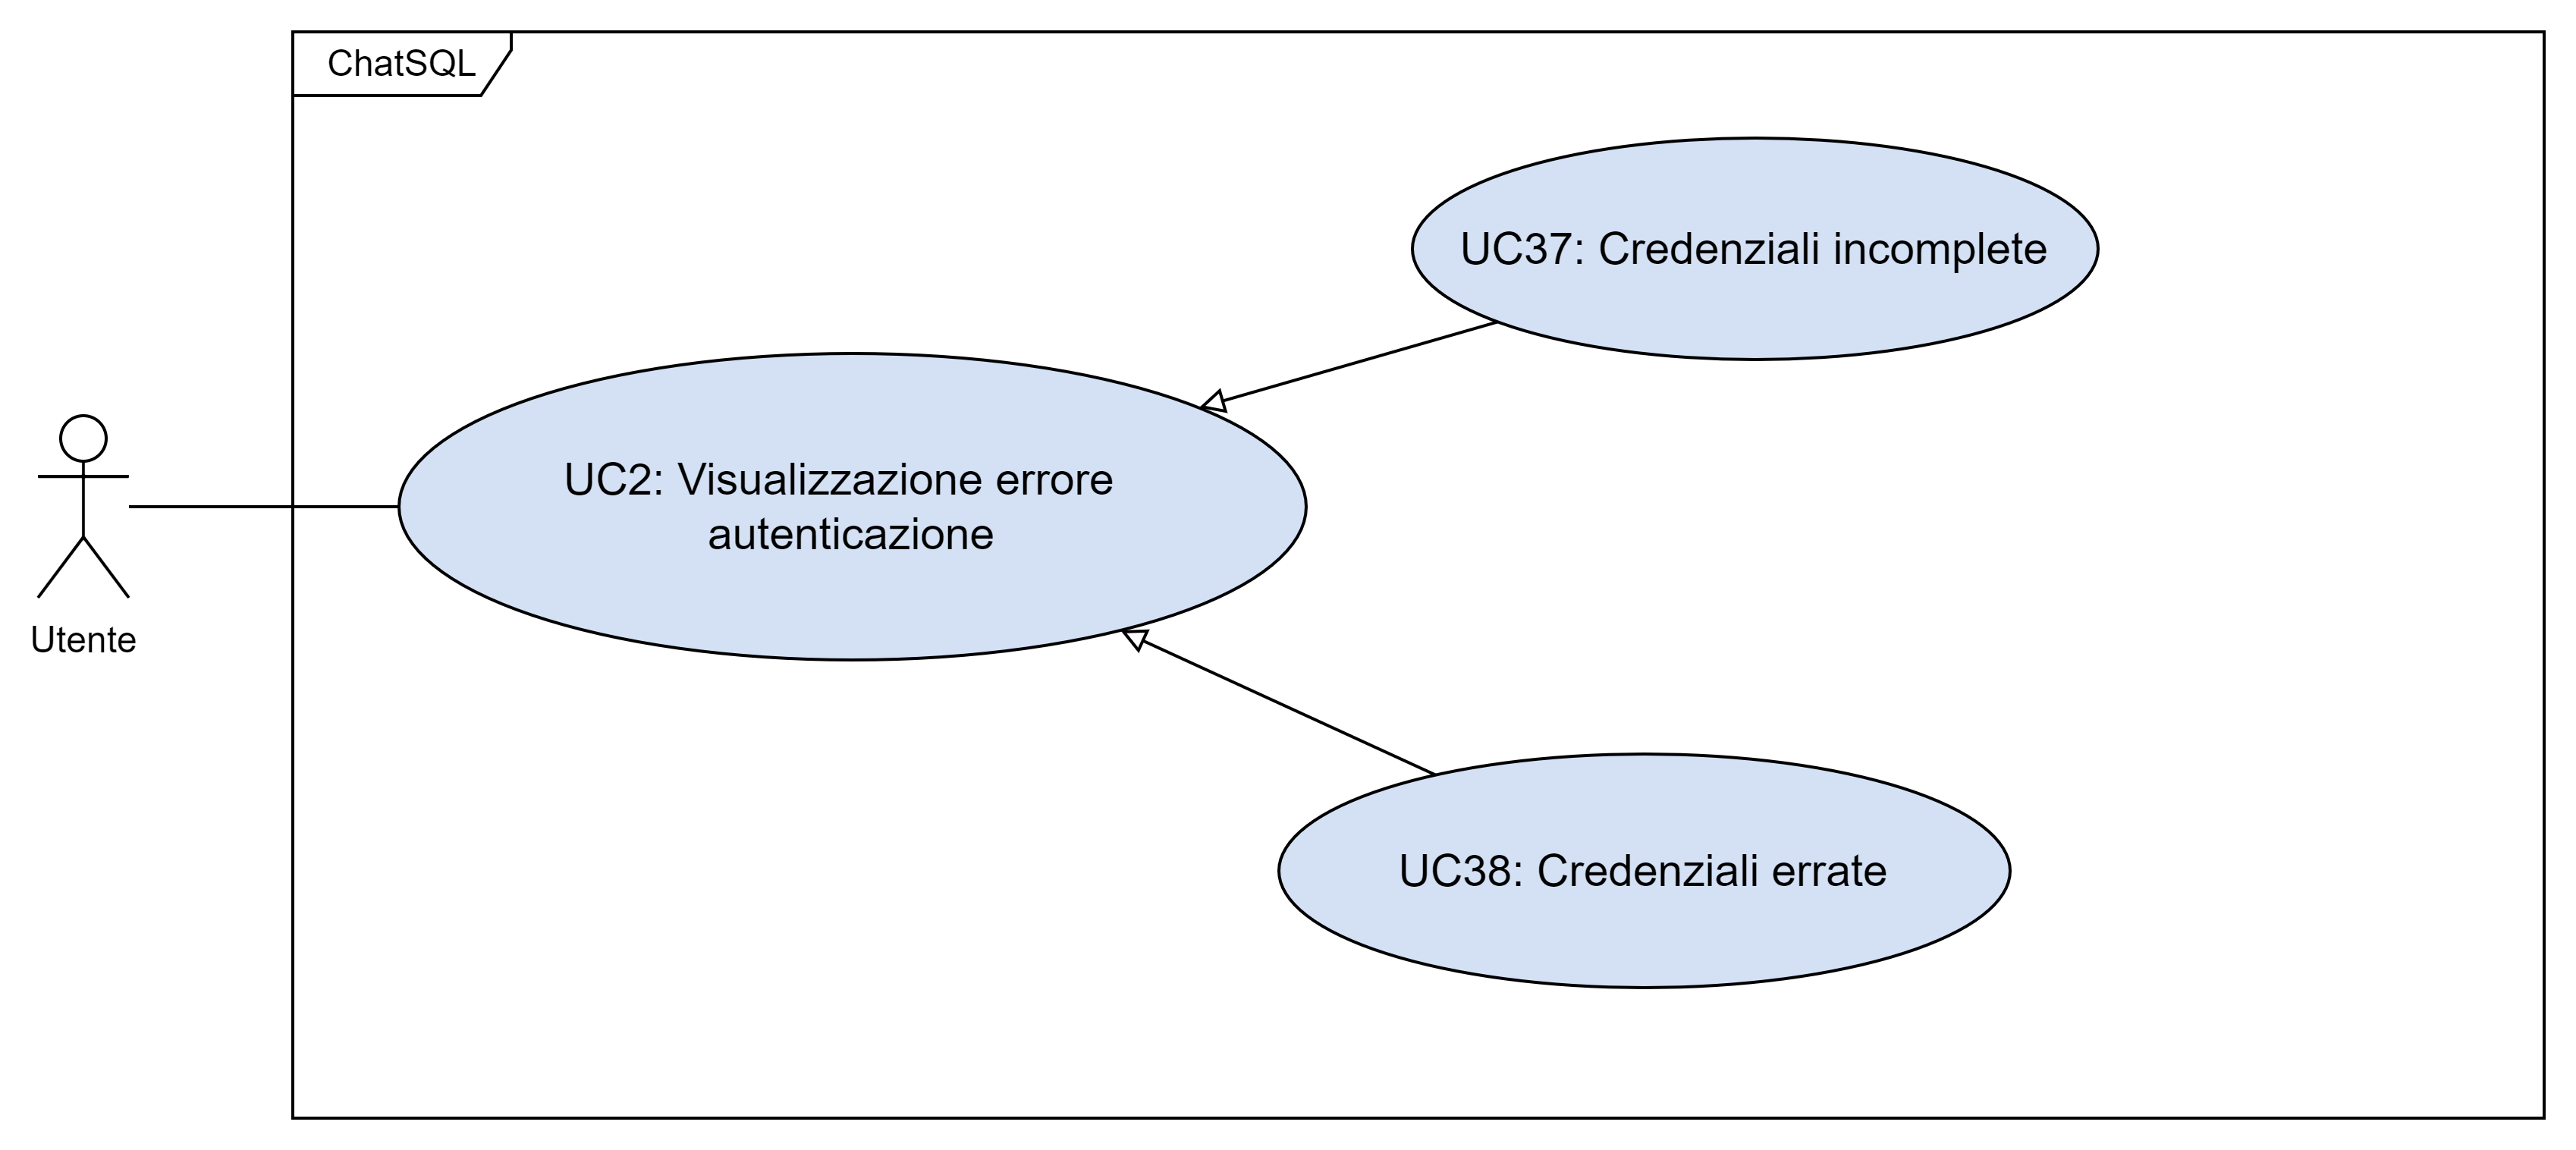
\includegraphics[width=0.90\textwidth]{assets/uc2.png}
  \caption{UC2}
\end{figure}

\paragraph*{Descrizione}
Al rilevamento da parte del sistema di irregolarità durante il processo di validazione delle credenziali al momento del login, degli appositi messaggi di errore informeranno l’Utente della natura del problema riscontrato.

\paragraph*{Attori principali}
Utente

\paragraph*{Precondizioni}
\begin{itemize}
  \item L’Utente ha inserito le proprie credenziali nell’area di login (\hyperref[UC1]{UC1});
  \item Il sistema ha riscontrato un problema nel processo di autenticazione.  
\end{itemize}

\paragraph*{Postcondizioni}
\begin{itemize}
  \item Viene mostrato un messaggio di errore per notificare l’Utente dell’incorretto o parziale inserimento dei dati nell’area di login.
\end{itemize}

\paragraph*{Scenario principale}
\begin{enumerate}
  \item L’Utente tenta di autenticarsi all’applicativo inserendo le proprie credenziali nell’area di login;
  \item Il sistema rileva lo scorretto o parziale inserimento delle credenziali;
  \item Viene segnalato all’Utente il messaggio d’errore relativo alla problematica riscontrata.  
\end{enumerate}

\paragraph*{Generalizzazioni}
\begin{itemize}
  \item Errore credenziali incomplete (\hyperref[UC2point1]{UC2.1});
  \item Errore credenziali errate (\hyperref[UC2point2]{UC2.2});
  \item Errore Utente non registrato (\hyperref[UC2point3]{UC2.3}).
\end{itemize}

%%%%%%%%%%%%%%%%%%%%%%%%%%%%%%%%%%%%%%%%%%%%%%%%%%%%%%%%%%%%%%%%%%%%%%%%%%%%%%

\subsubsection{UC2.1 - Errore credenziali incomplete}\label{UC2point1}
\paragraph*{Descrizione}
L’errore relativo all’incompletezza delle credenziali viene mostrato a seguito del rilevamento parziale delle credenziali inserite da parte dell’Utente.

\paragraph*{Attori principali}
Utente

\paragraph*{Precondizioni}
\begin{itemize}
  \item L’Utente non ha eseguito il login;
  \item L’Utente ha inserito solo il proprio username o la propria password come credenziali nel tentativo di autenticarsi.  
\end{itemize}

\paragraph*{Postcondizioni}
\begin{itemize}
  \item Viene mostrato un messaggio di errore per notificare l’Utente del parziale inserimento dei dati nell’area di login.
\end{itemize}

\paragraph*{Scenario principale}
\begin{enumerate}
  \item L’Utente ha inserito solo una delle due credenziali richieste durante il login;
  \item Il sistema mostra un messaggio di errore relativo al mancato inserimento dei dati di accesso all’applicativo.   
\end{enumerate}

%%%%%%%%%%%%%%%%%%%%%%%%%%%%%%%%%%%%%%%%%%%%%%%%%%%%%%%%%%%%%%%%%%%%%%%%%%%%%%

\subsubsection{UC2.2 - Errore credenziali errate}\label{UC2point2}
\paragraph*{Descrizione}
L’errore relativo alle credenziali errate viene mostrato in seguito all’inserimento di un username dal formato incorretto o della non corrispondenza tra username e password per un Tecnico registrato.

\paragraph*{Attori principali}
Utente

\paragraph*{Precondizioni}
\begin{itemize}
  \item L’Utente non ha eseguito il login;
  \item L’Utente ha tentato l’autenticazione con credenziali errate.  
\end{itemize}

\paragraph*{Postcondizioni}
\begin{itemize}
  \item Viene mostrato un messaggio di errore per notificare l’Utente dell’errato inserimento dei dati nell’area di login.
\end{itemize}

\paragraph*{Scenario principale}
\begin{enumerate}
  \item L’Utente ha tentato la procedura di login con credenziali errate;
  \item Il sistema mostra un messaggio di errore relativo all’errato inserimento dei dati di accesso all’applicativo.    
\end{enumerate}

%%%%%%%%%%%%%%%%%%%%%%%%%%%%%%%%%%%%%%%%%%%%%%%%%%%%%%%%%%%%%%%%%%%%%%%%%%%%%%

% Questo usercase viene modificato a seguito della presenza di una mancata corrispondenza tra username e password in UC2.2

\subsubsection{UC2.3 - Errore password errata}\label{UC2point3}
\paragraph*{Descrizione}
L’errore relativo all'inserimento di una password che non corrisponde a quella richiesta per l'accesso per l'username inserito per un Tecnico registrato.

\paragraph*{Attori principali}
Utente

\paragraph*{Precondizioni}
\begin{itemize}
  \item L’Utente non ha eseguito il login;
  \item L’Utente ha tentato l’autenticazione con un username corretto, ma una con una password errata.  
\end{itemize}

\paragraph*{Postcondizioni}
\begin{itemize}
  \item Viene mostrato un messaggio di errore per notificare l’Utente dell'inserimento di una password errata.
\end{itemize}

\paragraph*{Scenario principale}
\begin{enumerate}
  \item L’Utente ha tentato la procedura di login inserendo un username associato ad un account Tecnico, ma con una password non corrispondente per quell'utente;
  \item Il sistema mostra un messaggio di errore relativo all'inserimento errato della password.   
\end{enumerate}
